\section{Implementación}

\subsection[Lenguajes]{Lenguajes de programación}

Se han utilizado un total de 3 lenguajes distintos:

\begin{itemize}
	\item \textbf{Python}: El grueso de la implementación se ha realizado en
		este lenguaje de script. Se ha elegido debido a su sencillez y
		las ventajas que ofrecen mecanismos tales como las \textit{listas por
		comprensión}.
	\item \textbf{Bash}: Utilizado por ser la forma más directa y sencilla
		de utilizar tuberías de Linux.
	\item \textbf{Make}: Ancestral sistema de control de dependencias. Se
		caracteriza por la sencillez de su lenguaje y facilita
		enormemente la automatización de la generación y ejecución de
		las diversas partes del proyecto.
\end{itemize}

\subsection[Arquitectura]{Arquitectura del sistema}

El proyecto está dividido en varios módulos independientes que se pasan la
información a través de parámetros o archivos.

Los principales módulos \textit{Splitter}, \textit{Trainer}, \textit{Classifier}
y \textit{Evaluator} generan y reciben archivos. Debido a que van a realizarse
muchos tests, se ha optimizado este intercambio de información mediante el uso
de las \textbf{tuberías} que nos ofrece Linux. De esta forma la información
generada nunca llega a escribirse a disco: el módulo que la consume la recibe
directamente cuando el módulo que la genera la escribe en la tubería. Esto no
quita que se puedan utilizar sin ellas y de forma independiente.

En la figura~\ref{fig:esquema} se pueden observar los distintos módulos y el
flujo de información entre ellos. Las cajas representan a los módulos y las
elipses a los mensajes.

\begin{landscape}
\begin{figure}[p]
	\centering
	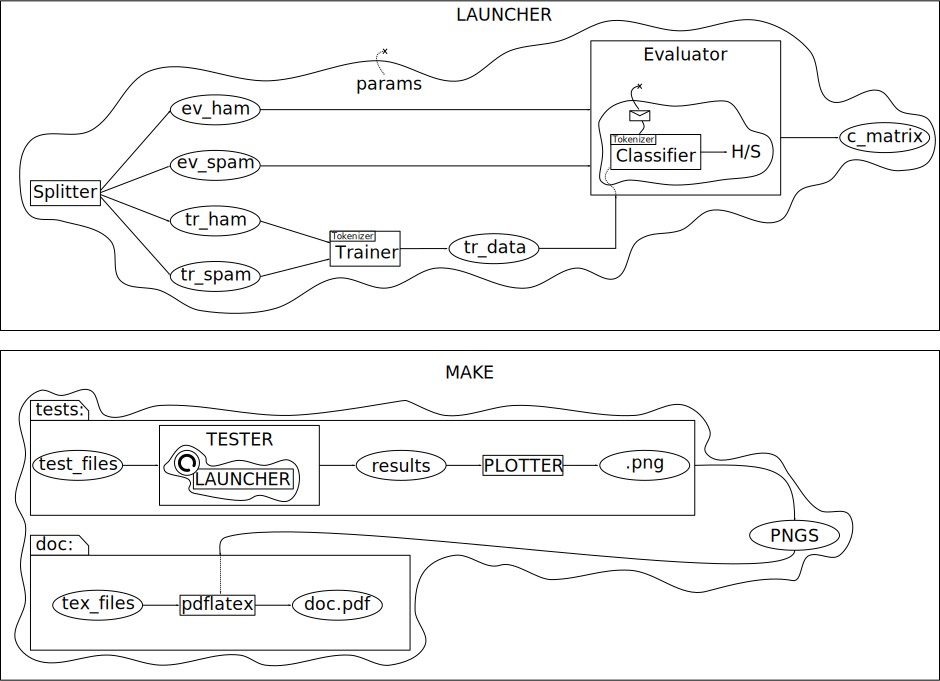
\includegraphics[width=\paperwidth, height=\paperheight, keepaspectratio]{img/esquema}
	\caption{Esquema de la arquitectura del sistema}
	\label{fig:esquema}
\end{figure}
\end{landscape}

\subsubsection{Splitter}

\begin{itemize}
	\item \textbf{Funcionalidad}: Extraer de la base de datos de correos los
		\textbf{conjuntos de evaluación y entrenamiento}
	\item \textbf{Parámetros}: Porcentajes del conjunto de evaluación y
		entrenamiento, o selección $enron[1-5] \rightarrow
		\text{entrenamiento},\ enron6 \rightarrow \text{evaluación}$
	\item \textbf{Entradas}: Base de datos de correos
	\item \textbf{Salidas}: 4 listas de rutas a correos: evaluación/spam,
		evaluación/ham y entrenamiento/spam
\end{itemize}

Éste módulo pasa las listas al \textit{Trainer} y al \textit{Evaluator} mediante
tuberías.

\subsubsection{Trainer}

\begin{itemize}
	\item \textbf{Funcionalidad}: Extraer características del conjunto de
		entrenamiento que permitan al clasificador distinguir entre un
		correo ham y uno spam
	\item \textbf{Parámetros}: Tipo de tokenización
	\item \textbf{Entradas}: Listas de rutas a correos de spam y de ham
	\item \textbf{Salidas}: Datos de entrenamiento con las características
		aprendidas
\end{itemize}

La salida del trainer se pasa al \textit{Evaluator} mediante una tubería.

\subsubsection{Classifier}

\begin{itemize}
	\item \textbf{Funcionalidad}: Clasificar un correo como spam o ham
	\item \textbf{Parámetros}: Umbral
	\item \textbf{Entradas}: Datos de entrenamiento y ruta del correo a
		clasificar
	\item \textbf{Salidas}: Una cadena: ``ham'' o ``spam''
\end{itemize}

\subsubsection{Evaluator}

\begin{itemize}
	\item \textbf{Funcionalidad}: Generar la matriz de confusión dado un
		conjunto de evaluación
	\item \textbf{Parámetros}: Umbral
	\item \textbf{Entradas}: Listas de rutas a correos de spam y de ham
	\item \textbf{Salidas}: Los cuatro números de la matriz de confusión en
		tanto por uno
\end{itemize}

\subsubsection{Tokenizer}

\begin{itemize}
	\item \textbf{Funcionalidad}: Dividir un correo en tokens (unidad mínima
		de división de un correo que consideramos que lo caracteriza)
	\item \textbf{Parámetros}: Estrategia de tokenización
	\item \textbf{Entradas}: Ruta al correo a tokenizar
	\item \textbf{Salidas}: Lista de tokens
\end{itemize}

Lo primero que se hace es eliminar los saltos de línea y pasar todo el texto a
minúsculas. A partir de aquí se siguen distintas \textbf{estrategias} de
tokenización:

\begin{itemize}
	\item \textbf{basic}: Toma palabras (números o letras) de 1 o más caracteres
	\item \textbf{word2}: Toma palabras (números o letras) de 2 o más caracteres
	\item \textbf{alphnum2}: Toma palabras (números o letras) con 2 o más letras
	\item \textbf{alphnum3}: Toma palabras (números o letras) con 3 o más letras
	\item \textbf{alph3}: Toma palabras con 3 o más letras
	\item \textbf{groupwords+alph3}: Toma palabras con 3 o más letras y
		cambia ciertas estructuras por tokens especiales
	\begin{itemize}
		\item \texttt{\_\_\_url\_\_\_}: Cada vez que se encuentra una
			URL se añade este token
		\item \texttt{\_\_\_spam\_word\_\_\_}: Se ha observado que es
			típico en los correos de spam encontrar palabras
			escritas con un espacio en cada letra. Cada vez que se
			encuentra una de estas palabras se sustituye por este
			token.
		\item \texttt{\_\_\_spam\_symbols\_\_\_}: Muchas exclamaciones
			seguidas, puntos y agrupaciones de símbolos extraños
			también son una característica de los correos de spam.
			Los sustituimos por este token
		\item \texttt{\_\_\_number\_\_\_}: El significado cuantitativo
			de un número no tiene relevancia a la hora de clasificar
			un correo, nos quedamos con el cualitativo utilizando
			este token.
	\end{itemize}
\end{itemize}

\subsubsection{Launcher}

\begin{itemize}
	\item \textbf{Funcionalidad}: Ejecutar la cadena
		\textit{splitter-trainer-evaluator} utilizando las tuberías de
		Linux
	\item \textbf{Parámetros}: Porcentajes de evaluación y entrenamiento,
		umbral y tipo de tokenización. Todos opcionales, si se omiten se
		toman valores por defecto
	\item \textbf{Entradas}: Ninguna
	\item \textbf{Salidas}: Una cadena con los siguientes elementos
		separados por `;' (pensados para ser parseados por el
		\textit{plotter}):
		\begin{equation*}
			<\text{valores de parámetros (si han modificado)}>;<m_1>;<m_2>;<m_3>;<m_4>
		\end{equation*}
		Donde $<m_i>$ son los elementos de la matrix de confusión
\end{itemize}

\subsubsection{Tester}

\begin{itemize}
	\item \textbf{Funcionalidad}: Ejecutar un \textit{test} y guardar los
		resultados
	\item \textbf{Parámetros}: Ninguno
	\item \textbf{Entradas}: Fichero de test
	\item \textbf{Salidas}: Un archivo con las salidas recogidas del
		\textit{Launcher}, una por línea.
\end{itemize}

\subsubsection{Plotter}

\begin{itemize}
	\item \textbf{Funcionalidad}: Crear un fichero \texttt{.png} con una
		gráfica que representa los resultados generados por el
		\textit{Tester}
	\item \textbf{Parámetros}: Nada
	\item \textbf{Entradas}: Fichero de resultados del \textit{Tester}
	\item \textbf{Salidas}: Gráfica en \texttt{.png}
\end{itemize}
